%priprava posamezne ure
%tukaj zaporedoma napisemo{st. zaporedne ure}{datum}{naslov}{poglavje}{oblika dela}{pripomocki}
\begin{priprava}{}{}{Zaporedja}{(Neskončne) vrste}{frontalna}{tabla}

Zaporedje: $ a_1, a_2, a_3, a_4 \ldots, a_n $ \\
Vrsta \didopomba{je vsota členov zaporedja}: $ a_1 + a_2 + a_3 + a_4 + \ldots + a_n $ \didopomba{lahko samo v zaporedju zbrišeš vejice in napišeš plus, je bolj nazorno}

Če seštevano vse člene neskončnega zaporedja, govorimo o \emph{neskončni} vrsti. Označimo:

$$ (S =) \ a_1 + a_2 + a_3 + a_4 + \ldots = \sum_{n=1}^{\infty} a_n $$
\didopomba{$ S $ je tu samo zaradi oznake, lahko je karkoli.}

Primeri:
\begin{itemize}
    \item Seštej zaporedje naravnih števil. \didopomba{ $ 1 + 2 + 3 + 4 + 5 + \ldots $ jasno gre v neskončnost.}
    \item Seštej vrsto $ 1 + 1/2 + 1/3 + 1/4 + 1/5 + \ldots $. \didopomba{Tukaj ni očitno, da vsota ni končna. Ali pa, saj vedno prišteješ nekaj zraven, in ker neskončnokrat prišteješ, bo pa ja šlo vse v neskončnost? Zato si pogledamo še konvergenten primer:}
    \item Ahil in želva tečeta v isto smer. Ahil štarta en kilometer pred želvo in teče 2-krat hitreje. Ali Ahil ujame želvo?\didopomba{Ustno in s premico v dveh barvah nakažeš njuno premikanje -- želva preteče pol Ahilove razdalje. Ahil vedno razpolovi novo razdaljo do 2 km. Ahil preteče $ 1 + 1/2 + 1/4 + 1/8 + \ldots $km Tu zdaj povzameš problematični vidik neskončne vrste. Načeloma je ne moreš prešteti, ker ne moreš v neskončnost seštevati, to ni smiselno (baje so Grki imeli s tem konceptom probleme). Ampak to ne pomeni, da seštevanje neskončno členov da neskončno vsoto. V nekaterih primerih (npr. v tem) lahko vsoti vseeno pripišemo smiselno vrednost.} Kdaj ujame želvo? Če pogledamo pod mikroskop, je ne ujame nikoli, ampak v limiti, praktično, pa jo seveda ujame pri 2 km.
    \begin{figure}[h]
        \centering
        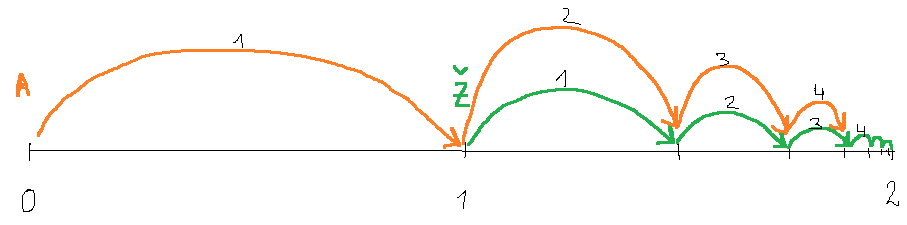
\includegraphics[width=\textwidth]{slike/ahil.png}
    \end{figure}
\end{itemize}

Vrste, ki se jih ne da sešteti (ne dobimo nič konkretnega), imenujemo \textbf{divergentne vrste}. Kako pa vemo, ali se da vrsto sešteti (takrat jo imenujemo \textbf{konvergentna vrsta})? Pogledamo \emph{delne vsote} \didopomba{Naj sami z malo vodenja vidijo, da moraš vzeti limito}:

\newpage

\begin{align*}
    S_1 & = a_1 \\
    S_2 & = a_1 + a_2 \\
    & \vdots \\
    S_n & = a_1 + \ldots + a_n \\
    & \vdots \\
    S & = \lim_{n \rightarrow \infty} S_n
\end{align*}

Če so delne vsote konvergentne, potem je vsota neskončne vrste enaka kar limiti delnih vsot. \didopomba{Lepe vrste za seštevanje so geometrijske vrste, zato si jih podrobneje poglejmo.}

\naslov{Neskončna geometrijska vrsta}

\didopomba{Našteješ zaporedja in naj vidijo, ali divergira ali ne. Konvergenten primer vzameš iz primera z Ahilom.}
\begin{itemize}
    \item $ 2 + 4 + 8+ 16 + \ldots $ divergira ($ q = 2 $)
    \item $ 1 - 1 + 1 - \ldots $ divergira ($ q = - 1 $)
    \item $ 1 - 3 + 9 - 27 + \ldots $ divergira ($ q = - 3 $)
    \item $ 2 + 1 + \frac{1}{2} + \frac{1}{4} + \ldots $ konvergira ($ q = \frac{1}{2} $)
\end{itemize}

Kdaj geometrijska vrsta konvergira?

$$
S = \lim_{n \rightarrow \infty} S_n = \lim_{n \rightarrow \infty} \frac{a_1 (q^n - 1)}{q - 1} = \lim_{n \rightarrow \infty} \frac{a_1 q^n - a_1}{q - 1} = \frac{a_1}{1 - q}
$$

\didopomba{Pred zadnjim enačajem si oglejmo število $ q^n $. Kam gre v limiti $ n \rightarrow \infty $? V neskončno, če $ |q| \geq 1 $, in v 0, če je $ |q| < 1 $. Zato slednje vzamemo za potreben pogoj in zapišemo še zadnji enačaj.}

\vaje{
Vaje:
\begin{itemize}
    \item Ahil začne teči na razdalji 100 m pred želvo. Je 10x hitrejši od želve. Kdaj jo dohiti? \\
    $ 100 + 10 + 1 + 1/10 + \ldots = 111,\overline{1}\ldots $
    \item izračun vsote s to formulo, kakšne enačbe (npr. za kateri x je vrsta konvergentna), lahko je dano zaporedje, lahko je dana vsota in drugi člen, obseg likov na slikci \ldots
    \item zapiši $ 4,\overline{12} $ z ulomkom \didopomba{$ = 4 + \frac{12}{100} + \frac{12}{100^2} + \ldots $, lahko pa po vsaki decimalki posebej in imaš dve vsoti. Nato še na način iz 1. letnika, da preveriš.}
    \item Poenostavi $ \sqrt{2\sqrt{2\sqrt{2\sqrt{2\sqrt{2\ldots}}}}} $ \didopomba{$ = 2^{1/2} + 2^{1/4} + 2^{1/8} + \ldots = 2 $, potem pa še na lažji način, če vse skupaj označiš z $ x $: $ x = \sqrt{2x} $.}
\end{itemize}
}

\didopomba{Omeni harmonično vrsto!!! Lahko napišeš programček, ki ti izračuna, koliko členov moraš sešteti, da dobiš vsoto večjo od x. Za katerokoli vsoto moraš dobiti nek x.}

\end{priprava}